\documentclass{article}
\usepackage[spanish]{babel}
\usepackage[table]{xcolor}
\usepackage[utf8]{inputenc}
\usepackage{anysize} %Margen
\usepackage{float}
\usepackage{graphicx} %imagenes
\usepackage{hyperref}
\usepackage{hyperref}
\usepackage{sectsty}
\usepackage{url}

\begin{document}
\marginsize{2cm}{2cm}{1cm}{2cm} 

\begin{center}
  {\LARGE \scshape Proyecto de Riesgo Tecnológico\\\vspace{10mm} }
  \rule{0.8\textwidth}{.8pt}\\
\end{center}

\section*{Empresa}

\subsection*{Nombre del equipo} \textit{\textbf{Vakas Lokas}}
\subsection*{Logo del equipo}
\begin{center}
  
\includegraphics[scale=.2]{../imagenes/logoo.png}
\end{center}
\subsection*{Slogan}
\begin{center}
  \textit{``¿En qué término prefiere su software?''}
                          
\end{center}

\rule{0.8\textwidth}{.8pt}\\

\subsection*{Misión}
Brindar servicios de software de buena calidad, analizando los riesgos que
podrían afectar a nuestros clientes.

\rule{0.8\textwidth}{.8pt}\\

\subsection*{Visión}
Apoyar, creer y motivar a cualquiera en el mercado que necesite de la tecnología.

\rule{0.8\textwidth}{.8pt}\\

\subsection*{Propósito}
Desarrollar proyectos de software que ayuden a la comunidad de la facultad de ciencias

\rule{0.8\textwidth}{.8pt}\\

\subsection*{Valores}

\begin{itemize}
\item Transparencia.
\item Puntualidad.
\item Responsabilidad
\item Pasión.
\item Resolución.
\end{itemize}

\rule{0.8\textwidth}{.8pt}\\

\subsection*{Involucrados}
\subsubsection*{Equipo de trabajo}
\begin{itemize}
\item Galeana Araujo Emiliano. 314032324 Responsable Técnico.
\item Jardines Mendoza César Eduardo. 314071549 Responsable de Calidad.
\item Mendoza Castillo María Fernanda. 314280587 Líder de equipo.
  
    Hemos sido equipo en otras materias de la carrera, en las cuales la persona
  (Fernanda) ha mostrado las mejores aptitudes y cualidades; Tales como la
  responsabilidad, el compañerismo y la ayuda a sus compañeros de equipo. Esto,
  aunado a los FODA's individuales fueron razones por las que decidimos votar por
  Fernanda para ser la líder de equipo.
\end{itemize}

\subsubsection*{Docentes}
\begin{itemize}
\item Profesor: Selene Marisol Martínez Ramírez
\item Ayudante: Arturo Castillo Valles
\item Ayud. Laboratorio: Luis Rey Rutiaga Robles
\end{itemize}

\rule{0.8\textwidth}{.8pt}\\

\subsection*{FODA}

\begin{center}
  \begin{table}[H]
    \centering
    \begin{tabular}{| c | c | }
      \hline
      \cellcolor{green!25}Organización de tiempo. & \cellcolor{yellow!25}Rápido aburrimiento. \\
      \cellcolor{green!25}Aprendizaje rápido. & \cellcolor{yellow!25}Encontrar distracciones. \\
      \cellcolor{green!25}Conocimiento de idiomas. & \cellcolor{yellow!25}Distraer a los demás. \\
      \cellcolor{green!25}Trabajo en equipo. & \cellcolor{yellow!25}Trabajar en ciertas condiciones. \\
      \cellcolor{green!25}Investigación de cosas. & \cellcolor{yellow!25}Disponibilidad de tiempo. \\
      \cellcolor{green!25}Creatividad & \cellcolor{yellow!25}Seguir un único camino. \\
      \cellcolor{green!25}Mentalidad de tiburón. & \cellcolor{yellow!25}Hedonismo.\\
      \cellcolor{green!25}Perseverancia. & \cellcolor{yellow!25}Difucultad al tomar desiciones.\\
      \cellcolor{green!25}Comprometido. & \cellcolor{yellow!25}Distracciones externas. \\
      \cellcolor{green!25}Constancia en lo que hacemos. & \cellcolor{yellow!25}Baja tolerancia a la frustración. \\
      \cellcolor{green!25}F & \cellcolor{yellow!25}D. \\ \hline
      \cellcolor{blue!25}Actividades extracurriculares. & \cellcolor{red!25}Compromisos familiares. \\
      \cellcolor{blue!25}Aprender cualquier cosa. & \cellcolor{red!25}Falta de tiempo. \\
      \cellcolor{blue!25}Diplomados. & \cellcolor{red!25}Hobbies. \\
      \cellcolor{blue!25}Amigos en distintas áreas. & \cellcolor{red!25}Que me inviten a salir. \\
      \cellcolor{blue!25}Conocer personas. & \cellcolor{red!25}Prioridades en otras cosas. \\
      \cellcolor{blue!25}Mejorar cosas del entorno.& \cellcolor{red!25}Prefiero hacer algo divertido. \\
      \cellcolor{blue!25}Estudiar otras cosas. & \cellcolor{red!25}Nuevos proyectos.\\
      \cellcolor{blue!25}Reposo. & \cellcolor{red!25}Aburrimiento.\\
      \cellcolor{blue!25}Abrir nuestro círculo social. & \cellcolor{red!25}Deseos. \\
      \cellcolor{blue!25}Cosas de interés. & \cellcolor{red!25}Estrés. \\
      \cellcolor{blue!25}O & \cellcolor{red!25}A\\ \hline
    \end{tabular}
    \caption{FODA del equipo.}
    \label{tabla:horarios}
  \end{table}
\end{center}



\rule{0.8\textwidth}{.8pt}\\

\newpage
\section*{Producto de Software}

\subsection*{Nombre del producto de software}
CafeCiencias\\

\rule{0.8\textwidth}{.8pt}\\

\subsection*{Metodología}
\subsubsection*{Desarrollo de Software}
\begin{itemize}
\item SCRUM
\item Kanban
\end{itemize}
\subsubsection*{Manejo de Riesgos}
\begin{itemize}
\item FODA
\item Diagrama de Tortuga
\end{itemize}

\rule{0.8\textwidth}{.8pt}\\

\subsection*{Periodo}
Fecha de inicio: 20 de Marzo de 2020\\
\indent Fecha de fin: 9 de Mayo de 2020\\


\rule{0.8\textwidth}{.8pt}\\

\subsection*{Repositorio común de documentos}
\href{https://sites.google.com/view/vakas-lokas/p\%C3\%A1gina-principal?authuser=1}{Página de la empresa}

\href{https://drive.google.com/open?id=13f9jp3Oli6AQF1Ap8VhoEKFXTPULumos}{RT-2020-Drive}

\href{https://github.com/mildewyPrawn/CafeCiencias}{RT-2020-Repositorio}

\href{https://trello.com/b/rwdAGuSi/cafeciencias}{RT-2020-Trello}

\rule{0.8\textwidth}{.8pt}\\

\subsection*{Propuesta de Proyecto Final}

“CafeCiencias” será una aplicación web destinada a las personas que suelen o
deseen ir a comer a la cafetería de la Facultad de Ciencias, así como el personal
de la cafetería. Esta aplicación ofrecerá una manera mas práctica y fácil de
saber los horarios, el menú de la comidas, sus precios, avisos y si alguna de las
comidas ya se  acabó. Además los usuarios podrán informar a otros sobre retrasos
en los horarios o la entrega de algunos platillos.

\rule{0.8\textwidth}{.8pt}\\

\subsection*{Casos de uso}

\begin{center}
  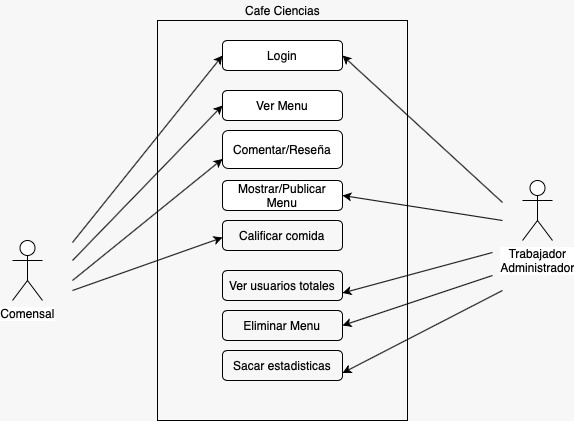
\includegraphics[scale=.75]{../imagenes/CasoDeUsos.jpg}
\end{center}

\rule{0.8\textwidth}{.8pt}\\

\subsection*{Propuesta de Valor}

La aplicación ofrece un acercamiento al momento entre la cafetería de la
Facultad con los clientes pues además de revisar al día los menús y precios,
habrá una discusión entre los mismos clientes para garantizar notificaciones
comunitarias en tiempo real evitando tener que ir a la cafetería.

\rule{0.8\textwidth}{.8pt}\\

\subsection*{Tipos de Usuarios}

La aplicación va dirigida en su mayoría a estudiantes, trabajadores y profesores
de la Facultad de Ciencias que disfruten de comer en la cafetería principal.
Aunque también pueden hacer uso de esta, personas que laboren en otra facultad,
instituto, dependencia de la UNAM. Y en casos extremos, personas ajenas a la
Universidad que gusten de comer ahí. 

El otro tipo de usuarios son trabajadores de la cafetería principal de la
facultad de ciencias, siendo ellos quienes actualizan el menú.

\rule{0.8\textwidth}{.8pt}\\

\subsection*{Tecnologías para la Implementación}

\begin{center}
  \begin{tabular}{| c | c | c | c | } \hline
    Concepto & Herramienta & Versión & Función \\\hline
    Framework & django & 2.2.4 & Para complementar funciones del lenguaje python. \\\hline
    Diagramador UML & draw.io & 11.2.8 &  Para realizar los diagramas \\\hline
    Manejador de bases de datos & sqlite3 & 3.31.1 & Para almacenar las bases de
    datos y operar con ellas. \\\hline
    IDE & Sublime & 3 & Para escribir \\
    & Emacs & 26.3 & código \\\hline
    Control de versiones & git & 2.23.0 & Para controlar las versiones y tener y \\
    & & & apoyarnos la producción del producto. \\ \hline
  \end{tabular}
\end{center}

\rule{0.8\textwidth}{.8pt}\\

\subsection*{Análisis de riesgos}
\subsubsection*{Cualitativos y cuantitativos}
\subsubsection*{Riesgos}
\begin{itemize}
\item Físicos
  \begin{itemize}
  \item Que explote el servidor.
  \end{itemize}
  
\item Humanos
  \begin{itemize}
  \item Sabotaje.
  \item Ataque informático.
  \item Que los administradores no publiquen un día.
  \item Que se borre la base de datos.
  \end{itemize}
    
\item Lógicos
  \begin{itemize}
  \item Que se permitan usuarios duplicados.
  \item Que un cliente pueda ingresar como administrador.
  \item Que no se pueda registrar/iniciar sesión.
  \end{itemize}
\end{itemize}
\subsubsection*{Diagrama de tortuga}
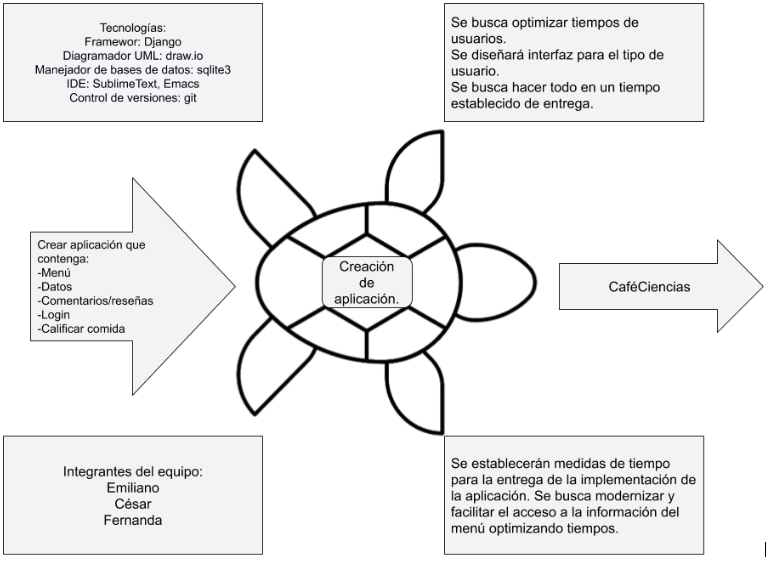
\includegraphics[scale=.5]{../imagenes/tortuga.png}

\subsubsection*{FODA}
%AGREGADO POR EL VAQUINENE
\begin{center}
  \begin{table}[H]
    \centering
    \begin{tabular}{| c | c | }
      \hline
      \cellcolor{green!25}Utilizado por muchos estudiantes. & \cellcolor{yellow!25}Uso de una conexión de internet estable. \\
      \cellcolor{green!25}Fácil de usar. & \cellcolor{yellow!25}Parte de los usuarios son externos. \\
      \cellcolor{green!25}Herramienta que optimiza tiempos. & \cellcolor{yellow!25}Puede ser no tan conocido entre la \\ 
      \cellcolor{green!25}& \cellcolor{yellow!25} comunidad fuera de la Facultad. \\
      \cellcolor{green!25}Provee información útil. & \cellcolor{yellow!25}Se puede volver monótona. \\
      \cellcolor{green!25}No necesita espacio. & \cellcolor{yellow!25}Es de uso muy rapido. \\
      \cellcolor{green!25}No necesita memoria & \cellcolor{yellow!25}Susceptible a errores humanos \\
      \cellcolor{green!25}Tiene una comunidad activa. & \cellcolor{yellow!25}No tener horario fijo de publicación.\\
      \cellcolor{green!25}Administrada por la Facultad & \cellcolor{yellow!25}No contar con certificado SSL\\
      \cellcolor{green!25}Gratis. & \cellcolor{yellow!25}Distracciones externas. \\
      
      \cellcolor{green!25}F & \cellcolor{yellow!25}D. \\ \hline
      \cellcolor{blue!25}Más gente contribuye a su uso. & \cellcolor{red!25}Que no se le de actualización . \\
      \cellcolor{blue!25}Modernizar. & \cellcolor{red!25}Falta de usuarios \\
      \cellcolor{blue!25}Nuevas funcionalidades. & \cellcolor{red!25}Que no tenga una buena interfaz de usuario. \\
      \cellcolor{blue!25}Más usuarios. & \cellcolor{red!25}No cuente con ergonomía. \\
      \cellcolor{blue!25}Mayor difusión. & \cellcolor{red!25}Que se tarde para algunos usuarios con poca conexión. \\
      \cellcolor{blue!25}Uso en cualquier explorador de internet y/o navegador. & \cellcolor{red!25}Capacitar a personas cada que se cambie de trabajadores. \\
      \cellcolor{blue!25}Optimizado a necesidades de los usuarios. & \cellcolor{red!25}Desuso.\\
      \cellcolor{blue!25}Adaptabilidad & \cellcolor{red!25}Falta de peronas que busquen mejorarlo para un mejor uso.\\
      \cellcolor{blue!25}O & \cellcolor{red!25}A\\ \hline
    \end{tabular}
    \caption{FODA del producto.}
    \label{tabla:horarios}
  \end{table}
\end{center}
\subsubsection*{What if?}
¿Qué pasaría si...
\begin{enumerate}
\item Se cae el servidor?
\item Si se roban los datos?
\item Cierran la cafetería?
\item Un día no hay servicio?
\item Un día no publica el administrador?
\item No hay trabajadores un día?
\item Dejan de ir a comer a la cafetería?
\item Si no se puede acceder a la página?
\item Quieren extender las funcionalidades?
\item La empiezan a usar para cosas inadecuadas?
\end{enumerate}

\subsubsection*{Cinco porqués}
\begin{enumerate}
\item ¿Por qué usar cafeCiencias?

  Porque apoya a los estudiantes que quieren comer en la facultad de Ciencias.
  
\item ¿Por qué?

  Porque pueden ver el menú de cada día y los comentarios.
  
\item ¿Por qué?

  Porque los administradores publican el menú y los usuarios los comentarios.
  
\item ¿Por qué?

  Para informar a los estudiantes que no están presentes en la cafetería del
  menú.
  
\item ¿Por qué?

  Porque hay alumnos que suelen comer en la cafetería pero cuando llegan ya no
  hay comida o tienen que decidir qué comer.
  
\end{enumerate}
\rule{0.8\textwidth}{.8pt}\\

\subsection*{Reuniones del equipo}

\rule{0.8\textwidth}{.8pt}\\

Cronograma del equipo por semana:\\
Semana 1 - 29 de marzo al 4 de abril \\
Semana 2 - 12 de abril al 18 de abril \\
Semana 3 - 19 de abril al 25 de abril \\
Semana 4 - 26 de abril al 2 de mayo \\
\begin{center}
  \begin{table}[H]
    \centering
    \begin{tabular}{| c | c | c | c | c | c | c | c | }
      \hline
      Actividad & Semana 1 & Semana 2 & Semana 3 & Semana 4 & Semana 5  \\
      \hline
      Página Web & 2hr & & & &  \\ \hline
      Revisión de idea & 1hr & & & &    \\ \hline
      Establecimiento de objetivos &  & &  & &   \\ \hline
      Reconocimiento de Contexto & 1hr & &  & &   \\ \hline
      Contextualizar diseño & 20min & &  & &   \\ \hline
      Implementación & & &  & &   \\ \hline
    \end{tabular}
    \caption{Cronograma por semana.}
    \label{tabla:horarios}
  \end{table}
\end{center}

\rule{0.8\textwidth}{.8pt}\\

Cronograma del equipo Semana 1 (29 de marzo a 4 de abril)
\\

\begin{center}
  \begin{table}[H]
    \centering
    \begin{tabular}{| c | c | c | c | c | c | c | c | }
      \hline
      Actividad & Lunes  & Martes  & Miercoles  & Jueves  & Viernes  & Sabado & Domingo  \\
      \hline
      Página Web & & & & 2hrs & & & \\ \hline
      Revisión de idea & & 1hr & & & & &    \\ \hline
      Establecimiento de objetivos &  & &  & & & &  \\ \hline
      Reconocimiento de Contexto & & & 1hr & & & & \\ \hline
      Contextualizar diseño & 20min & &  & & & &  \\ \hline
      Implementación &  & &  & & & &  \\ \hline
    \end{tabular}
    \caption{Cronograma por semana.}
    \label{tabla:horarios}
  \end{table}
\end{center}

\rule{0.8\textwidth}{.8pt}\\

Cronograma del equipo Semana 2 (12 de abril a 18 de abril)
\\

\begin{center}
  \begin{table}[H]
    \centering
    \begin{tabular}{| c | c | c | c | c | c | c | c | }
      \hline
      Actividad & Lunes  & Martes  & Miercoles  & Jueves  & Viernes  & Sabado & Domingo  \\
      \hline
      Página Web & & & & & & & \\ \hline
      Revisión de idea & & & & & & &    \\ \hline
      Establecimiento de objetivos & 2hrs & &  & & & &  \\ \hline
      Reconocimiento de Contexto & 20min & & & & & & \\ \hline
      Contextualizar diseño & 15min & &  & & & &  \\ \hline
      Implementación & & &  & & & &  \\ \hline
    \end{tabular}
    \caption{Cronograma por semana.}
    \label{tabla:horarios}
  \end{table}
\end{center}

\rule{0.8\textwidth}{.8pt}\\

\end{document}
